El detector TRITIUM, de la mateixa manera que el veto actiu del sistema de rebuig del fons radioactiu, consisteix en tres elements. El plàstic centellejador, que genera fotons en l'espectre visible com a resposta a la detecció d'una partícula, ja siga un decaïment del triti a la mostra o un esdeveniment del fons radioactiu. Els fotosensors, que detecten aquests fotons visibles i, com a conseqüència, generen un pols elèctric. L'electrònica, encarregada de processar i analitzar aquests polsos elèctrics. A la Figura \ref{fig:EsquemaDetector} es pot veure un esquema del detector descrit.

\begin{figure}[hbtp]
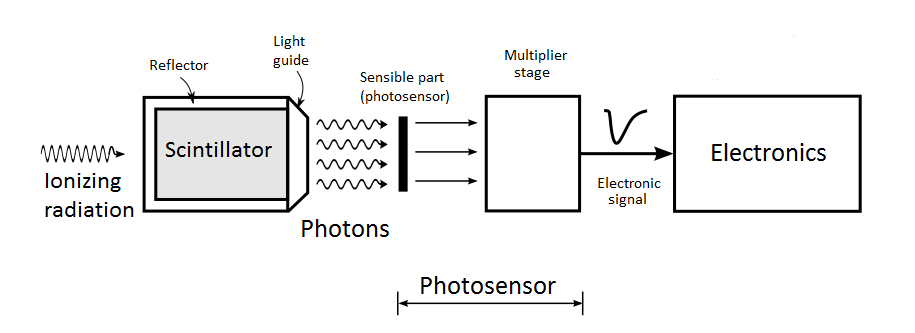
\includegraphics[scale=0.6]{12Summary/3DesignPrinciples/32Tritium_detector/ScintillatorDetector.png}
\centering
\caption{Esquema d'un detector de centelleig.\label{fig:EsquemaDetector}}
\end{figure}